\chapter{\babTiga}

% \todo{tambahkan kata-kata pengantar bab 1 disini}


% %-----------------------------------------------------------------------------%
% \section{Satu Persamaan}
% %-----------------------------------------------------------------------------%

% \noindent \begin{align}\label{eq:garis}
% 	\cfrac{y - y_{1}}{y_{2} - y_{1}} = 
% 	\cfrac{x - x_{1}}{x_{2} - x_{1}}
% \end{align}

% \equ~\ref{eq:garis} diatas adalah persamaan garis. 
% \equ~\ref{eq:garis} dan \ref{eq:bola} sama-sama dibuat dengan perintah \bslash
% align. 
% Perintah ini juga dapat digunakan untuk menulis lebih dari satu persamaan. 

% \noindent \begin{align}\label{eq:bola}
% 	\underbrace{|\overline{ab}|}_{\text{pada bola $|\overline{ab}| = r$}} 
% 		= \sqrt[2]{(x_{b} - x_{a})^{2} + (y_{b} - y_{a})^{2} + 
% 				\vert\vert(z_{b} - z_{a})^{2}}
% \end{align}

% %-----------------------------------------------------------------------------%
% \section{Lebih dari Satu Persamaan}
% \label{sec:multiEqu}
% %-----------------------------------------------------------------------------%
% \noindent \begin{align}\label{eq:matriks}	
% 	|\overline{a} * \overline{b}| &= |\overline{a}| |\overline{b}| \sin\theta 
% 		\\[0.2cm]
% 	\overline{a} * \overline{b} &=  
% 		\begin{array}{| c c c |}
% 			\hat{i} & x_{1} & x_{2} \\
% 			\hat{j} & y_{1} & y_{2} \\
% 			\hat{k} & z_{1} & z_{2} \\
% 		\end{array} \nonumber \\[0.2cm]
% 	&= \hat{i} \,
% 		\begin{array}{ | c c | }
% 			y_{1} & y_{2} \\
% 			z_{1} & z_{2} \\
% 		\end{array} 
% 	   + \hat{j} \,
% 		\begin{array}{ | c c | }
% 			z_{1} & z_{2} \\
% 			x_{1} & x_{2} \\
% 		\end{array} 
% 	   + \hat{k} \,	
% 		\begin{array}{ | c c | }
% 			x_{1} & x_{2} \\
% 			y_{1} & y_{2} \\
% 		\end{array}
% 		\nonumber
% \end{align}

% Pada \equ~\ref{eq:matriks} dapat dilihat beberapa baris menjadi satu bagian 
% dari \equ~\ref{eq:matriks}. 
% Sedangkan dibawah ini dapat dilihat bahwa dengan cara yang sama, \equ~
% \ref{eq:gabungan1}, \ref{eq:gabungan2}, dan \ref{eq:gabungan3} memiliki nomor 
% persamaannya masing-masing. 

% \noindent \begin{align}\label{eq:gabungan1}	
% 	\int_{a}^{b} f(x)\, dx + \int_{b}^{c} f(x) \, dx = \int_{a}^{c} f(x) \, dx
% 		\\\label{eq:gabungan2}
% 	\lim_{x \to \infty} \frac{f(x)}{g(x)} = 0 \hspace{1cm} 
% 		\text{jika pangkat $f(x)$ $<$ pangkat $g(x)$} \\\label{eq:gabungan3}
% 	a^{m^{a \, ^{n}\log b }} = b^{\frac{m}{n}}
% \end{align}

\section{Project Effort Estimation}

Untuk melakukan perhitungan project effort estimation, dapat dilakukan teknik Use Case Point (UCP) Estimation. Namun sebelum itu, dibuatkan use case diagram terlebih dahulu untuk memudahkan penentuan bobot dalam pembuatan UCP Estimation. Use case diagram  untuk Sistem dari Network Automation yang akan dibuat dapat dilihat pada gambar \ref{fig:usecase_diagram_ucp}.

\begin{figure}
	\centering
	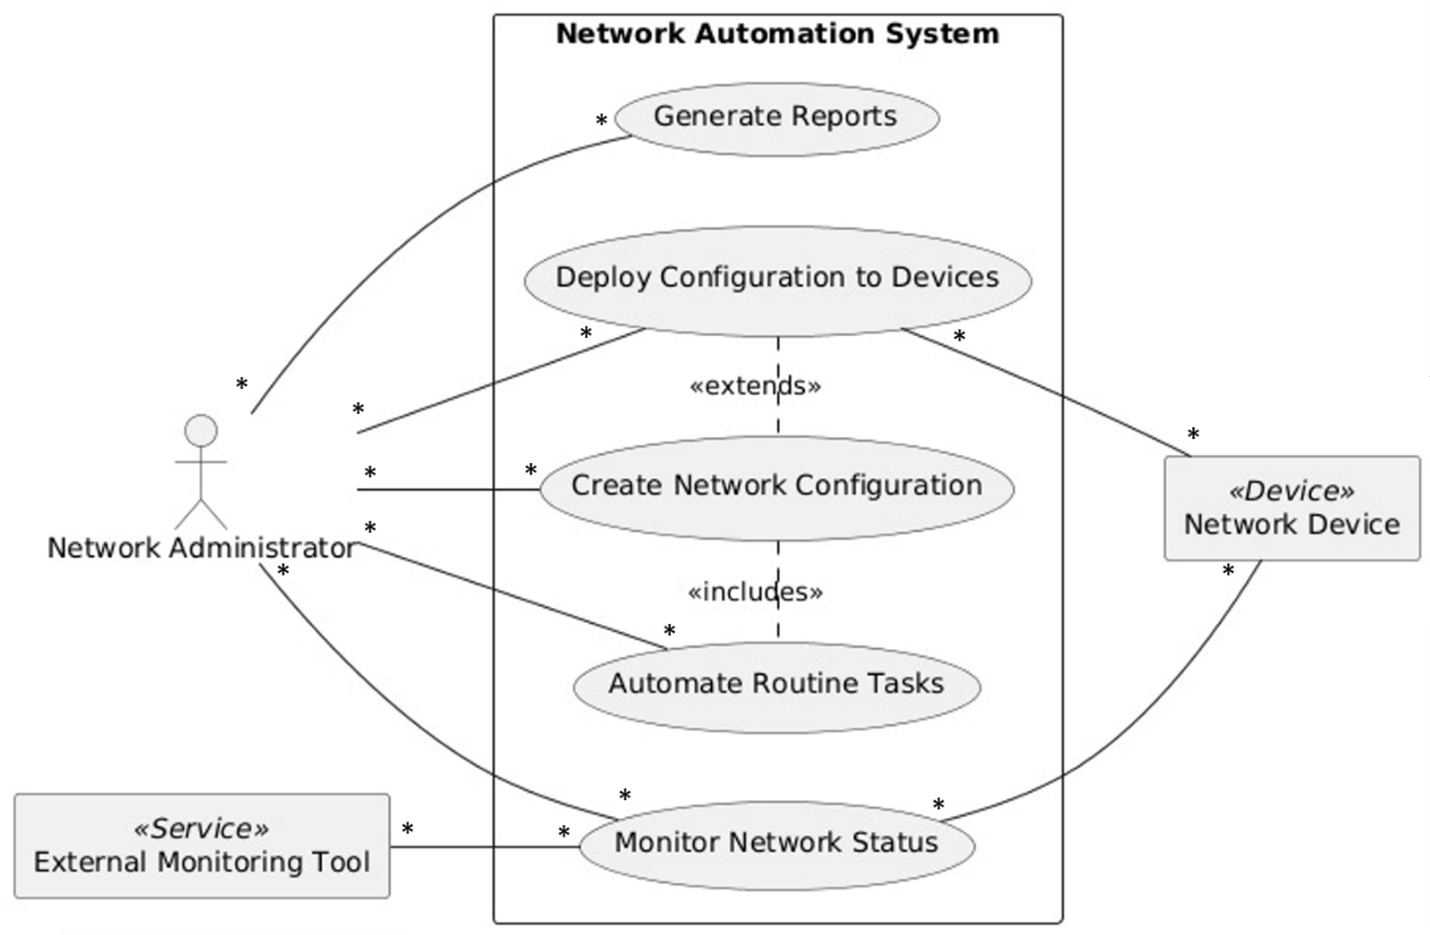
\includegraphics[width=0.70\textwidth]
		{assets/pics/usecase_diagram.png}
	\caption{Usecase diagram}
	\label{fig:usecase_diagram_ucp}
\end{figure}


\todo{elaborasi ttg ucp}



\section{Work Breakdown Structure}

\todo{pilih model, mau waterfall agile etc}
\todo{buat wbs-nya}


\section{Gantt Chart}

\todo{insert gantt chart}


\section{Staffing Plan}

\subsection{Peran dan Tanggung Jawab}


\todo{Isi staffing plan, isinya tree dari tim, peran masing2, tanggung jawab, persyaratan, jumlah staff, durasi kerja}


\subsection{Estimasi Biaya}

